\documentclass[11pt]{book}

\usepackage[authoryear]{natbib}
\usepackage{xcolor}
\usepackage[T1]{fontenc}
\usepackage{fourier}
\usepackage[utf8]{inputenc}
\usepackage[hidelinks]{hyperref}
\usepackage{slashbox}
\usepackage{graphicx}
\usepackage{url}
\usepackage{enumitem}


\newcommand{\todo}[1]{\textcolor{red}{[TODO: #1]}\PackageWarning{TODO:}{#1!}}
\newcommand{\note}[1]{\textcolor{red}{[NOTE: #1]}\PackageWarning{NOTE:}{#1!}}
\newcommand*{\np}{\par\noindent\newline}

\title{Agent Based Models of the Formation of Social Preferences}
\author{S Pardy}
\begin{document}
\begin{titlepage}
	\newcommand{\HRule}{\rule{\linewidth}{0.5mm}} % Defines a new command for horizontal lines, change thickness here
	
	\center % Centre everything on the page
	
	%------------------------------------------------
	%	Headings
	%------------------------------------------------
	
	\textsc{\LARGE Monash University}\\[1.5cm]	
	\textsc{\Large Bachelor of Science (Honours)}\\[0.5cm] % Major heading such as course name
	
	\textsc{\large Computational Science}\\[0.5cm] % Minor heading such as course title
	
	%------------------------------------------------
	%	Title
	%------------------------------------------------
	
	\HRule\\[0.4cm]
	
	{\huge\bfseries Agent Based Models of the Formation of Social Preferences}\\[0.4cm]
	
	\HRule\\[1.5cm]
	
	%------------------------------------------------
	%	Author(s)
	%------------------------------------------------
	
	\begin{minipage}{0.4\textwidth}
		\begin{flushleft}
			\large
			\textit{Author}\\
			Sam \textsc{Pardy}
		\end{flushleft}
	\end{minipage}
	~
	\begin{minipage}{0.4\textwidth}
		\begin{flushright}
			\large 
			\textit{Student ID}\\
		25940783   
		\end{flushright}
	\end{minipage}
	\vfill
	\vfill
	{\large
	\textit{Supervisor}\\
	Dr. Julian \textsc{Garcia}}
	
	%------------------------------------------------
	%	Date
	%------------------------------------------------
	
	\vfill\vfill\vfill % Position the date 3/4 down the remaining page
	
	{\large\today} % Date

	\vfill % Push the date up 1/4 of the remaining page
	
\end{titlepage}
% \hypersetup{colorlinks, citecolor=black, filecolor=black, linkcolor=black urlcolor=black}

% \newpage
% \chapter*{Declaration}
% \chapter*{Abstract}
% \chapter*{Acknowledgment}

\tableofcontents
\newpage
\chapter{Introduction}
\section{Preamble}
\section{Motivation \& Objectives}

\chapter{Literature Review}

\chapter[Theoretical \& Experimental Context]{Limitations of Theory \& The Experimental Framework}

The research discussed in the previous chapters suffers from several limitations that affect the generality of the conclusions drawn. 
Chiefly, it is static; the conclusions focus on evolutionary stable strategies as a solution concept.
These conclusions may be meaningful however do not tell us anything about how likely these strategies are to evolve or what circumstances may lead to them evolving.
Further, the work is slightly abstract in that in places it does not detail specific attributes of the model it is working with in favour of broader `catch-all' definitions,
this has made the process of creating software-based replicas of the models difficult at times.
The experimental framework that we have created as part of \textit{this} research seeks to recreate these models as dynamically-evolving before attempting to recover the results achieved in existing, static work.

\section{Limitations of Theory}
\np The primary source of theoretical work that this research has been on based is that of Alger \& Weibull (\citet{alger_generalization_2012}, \citet{alger_homo_2013}).
This work finds that under certain assumptions a utility function that is centred around a linear relationship between the two players' payoffs results in evolutionarily stable play.
This utility function is given in equation \ref{linearESSEquation}, in which \textit{x} and \textit{y} are types in the population and $\alpha$ is equal to the \textit{index of assortativity}.
\begin{equation}
	\label{linearESSEquation}
	\Pi_x(x, y, r) = \pi(x,y) + \alpha\pi(y,x)
\end{equation}

\noindent To achieve this, the authors assume that all types have a utility function of same form as \ref{linearESSEquation} where $\alpha \in (-1, 1)$ \citep[p. ~47]{alger_generalization_2012}.
This assumption severely limits the search space of the evolutionary process. The experimental framework that we have created in support of our research does not maintain this assumption.

\np A further assumption made in this work is that while players do not have information about their opponent's preferences,
the players converge to "mutually compatible" strategies and, in effect, play a Nash equilibrium with perfect information \citep[p. ~46]{alger_generalization_2012}.
It is unclear how controversial this assumption is. 
As discussed in previous chapters, it does not make sense to assume that players would have knowledge about their opponent's preferences 
but it may be acceptable to assume that when engaging in repeated interactions players converge to Nash equilibrium play relatively quickly.
However, it is possible that this assumption impacts the evolutionarily process substantially. Our experimental framework relies on this assumption also.

\np Commonly in the literature it is assumed that the agents will be matched to play symmetric, two-player games.
This is true also of \citet{alger_generalization_2012}.
In general, a \textit{symmetric} two-player game entails that an agent is indifferent (in terms of payoffs) as to which of the players she takes the roles of in the interaction.
This assumption makes easier our job of implementing a fitness-comparison mechanism.
As fitness is linked to the respective payoff achieved by each agent, the fact that the net payoff on offer to each player is equal simplifies the eventual fitness comparison.
However, we will see later that this assumption may have contributed to some bias in the sampling.

\np A final assumption to note is that the fitness used in the model in \citet{alger_generalization_2012} is that of \textit{average} fitness.
This measure is less stringent than measures used elsewhere (notably in \citet{alger_homo_2013}). 
An oft used fitness measure requires that for an invasion to occur, a mutant must achieve a higher payoff in all equilibria of all games the two types play when they're matched.

\np Of course, these assumptions are all made within the context of a model that is static.
The conclusions drawn in the work referenced above tend to be of the form \textit{should} a utility function of the form \textit{x} evolve it will result in evolutionary stable play given the assumptions.
The experimental framework we create intends to investigate these conclusions in a dynamically evolving environment.



\section{The Experimental Framework}
A large part of the work undertaken in support of this research involved the creation of an experimental framework that could be used to attempt to recover the results of \citet{alger_generalization_2012} in a dynamically evolving environment.
At a high level this experimental framework is simple, however when digging into the detail, complications arise.
Fundamentally, the framework is made up of a representation of a utility function, 
a means by which instances of this representation can be mutated and a means by which the fitness of two different utility functions can be compared.
With these building blocks we can construct the main loop of the experiments that are undertaken.
We define some utility function that represents our initial resident agent, the resident is then mutated (creating the mutant). 
The fitnesses of both resident and mutant are then computed and compared. 
If the mutant achieves a higher payoff an invasion occurs: the original resident is discarded and the mutant takes over as the new resident.
This process is repeated for a given number of generations.
In the following, we discuss the implementation detail of each of these fundamental parts of the framework, beginning with fitness.


\paragraph{Fitness}
\np Decisions we make about how we measure fitness and what difference in fitness is enough to trigger an invasion can have significant impact on the dynamics of the system.
This is an area in which Alger \& Weibull give us limited but essentially sufficient guidance.
Fitness is measured as the \textit{personal payoff} earned by each type when both players act in accordance with their own preferences.
For an individual $\theta$ in a population state $(\theta, \theta', \epsilon,\sigma)$,
where $\theta'$ is the mutant, $\epsilon$ is the mutant share of the population and $\sigma$ is the \textit{index of assortativity}, the expected fitness for one interaction is given by \ref{expectedPayoff}.
Where $f(x, y)$ is the expected payoff earned by $x$ when facing $y$ in a given iteration.

\begin{equation}
	\label{expectedPayoff}
	\Pi(\theta, \theta', \epsilon, \sigma) = (\sigma +(1-\epsilon)(1-\sigma))f(\theta, \theta) + \epsilon(1-\sigma)f(\theta, \theta')
\end{equation}

\np The notion of evolutionary stability is defined as follows: for a state to be considered stable, the residents must achieve, \textit{on average}, a fitness at least as high as that achieved by the mutants in a population that contains both resident and mutant types.
Using \ref{expectedPayoff}, this relation is given by \ref{ESSweakInequality}.
\begin{equation}
	\label{ESSweakInequality}
	F(\theta, \theta', \epsilon, \sigma) \geq F(\theta', \theta, \epsilon, \sigma)
\end{equation}
In other words, if inequality \ref{ESSweakInequality} does not hold, an invasion occurs.

Fitness in our source material, \citet{alger_generalization_2012}, is : for a population state to be considered \textit{unstable} the resident must achieve a payoff strictly less than that achieved by the mutant.
In practice, in our simulations, to calculate fitness we pit two utility surfaces (the resident and mutant) against one another and calculate the expected payoffs for each.
This is done with some population structure, $\epsilon$ in mind. So the expected payoff of the resident is given by:
\begin{equation}
\Pi(r, m, \epsilon) = (1-\epsilon)\pi(r,r) + \epsilon\pi(r,m)
\end{equation}

\paragraph{Games}
\np A key part of any game-theoretic model that attempts to represent the process of preference formation, is the kinds of games that are played.
For the most part, our source material (\citet{alger_generalization_2012}, \citet{alger_homo_2013}, \citet{newton_preferences_2017}) is largely agnostic about the games that are played in the models the work describes.
This work assumes only that the games are symmetric and two player. 
With this minimal assumption in mind, and given that we are interested in how cooperative preferences can develop we begin with a model in which the players are matched to play a single type of non-cooperative game.
It is quickly apparent that a fitness measure that is determined by the players' expected payoff in only one game does not yield generally meaningful results.
For example, using a prisoner's dilemma type we can write down a game with the payoff structure detailed in figure \ref{prisoners_payoff_matrices}.

\np When running simulations in which each type's fitness is determined by their expected payoff when playing the above game,
it becomes clear that only mutations that occur near to the payoff points ever lead to invasions. 
The payoff points are the four potential outcomes (in terms of payoffs for each player) of the game: (3,3), (0,4), (4, 0) \& (1, 1).
Plotted in figure \ref{prisoners_payoff_plot}.

\begin{figure}
	\centering
	\begin{tabular}{|l||*{5}{c|}}\hline
	 \label{prisoner_payoff}
	 \backslashbox{Prisoner A}{Prisoner B}
	 &\makebox[7em]{Remain Silent}&\makebox[7em]{Talk}\\\hline\hline
	 Remain Silent & 3, 3 & 0, 4\\\hline
	 Talk & 4, 0 & 1, 1 \\\hline
	 \end{tabular}
	 \caption{Payoff matrices detailing a prisoner's dilemma game.}
	 \label{prisoners_payoff_matrices}
\end{figure}\mbox{}\\

\begin{figure}
	\centering
	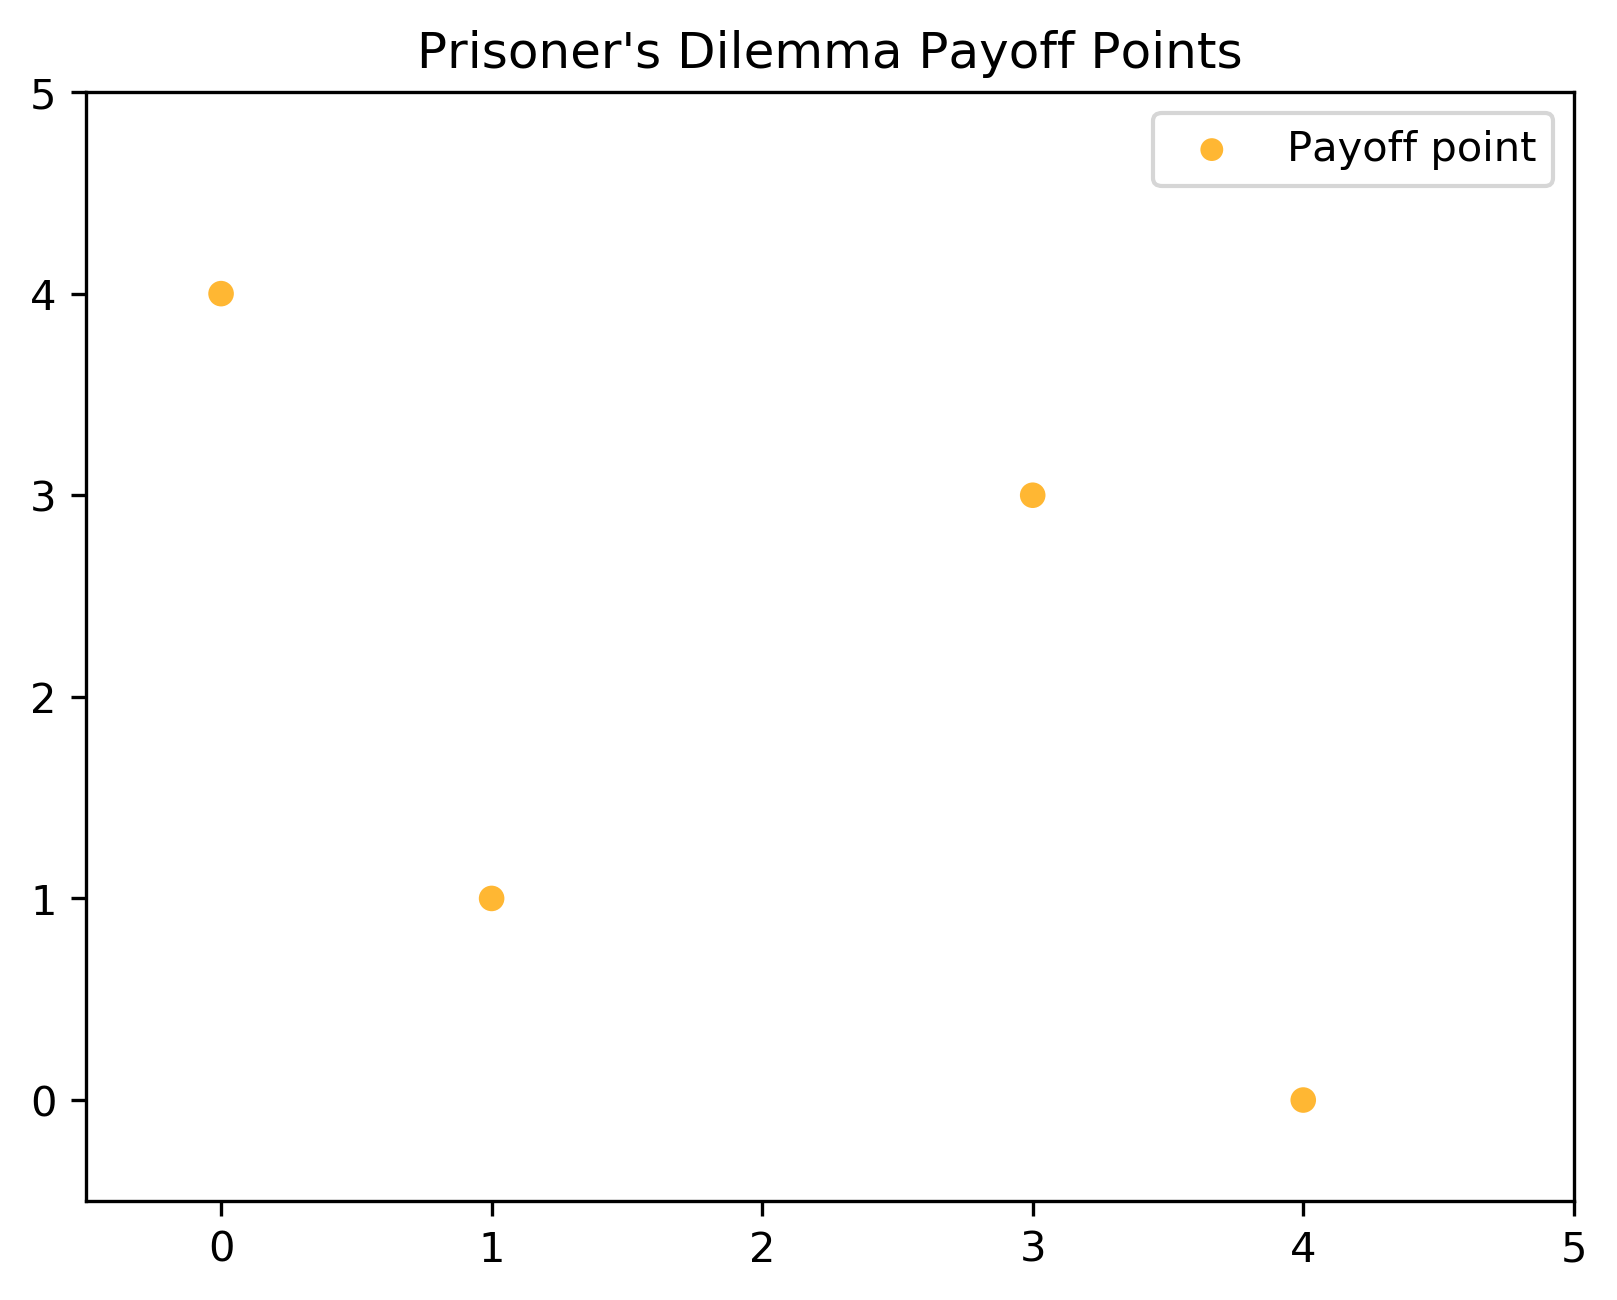
\includegraphics[scale=0.75]{resources/prisoners_dilemma_payoffs.png}
	\caption{The payoff points in a prisoner's dilemma game.}
	\label{prisoners_payoff_plot}
\end{figure}

\np The fact that limited invasions occur in this scenario makes sense when several facts about the model are considered:
\begin{enumerate}[label=(\alph*)]
	\item mutations can occur anywhere within the space and are small.
	\item the fitness of the agents (resident and mutant) is equal in areas of the surface not affected by the mutation.
	\item for a mutant to invade, they must achieve a fitness \textit{greater} than that achieved by the resident - as opposed to greater than or equal to.	
\end{enumerate} 
\np
So, if a mutation occurs at the point (2, 2), given that this mutation has a relatively small radius, 
the expected payoff of the mutant will not differ from that of the resident because the mutation does not touch any of the payoff points.
Hence, the fitnesses are equal, and no invasion occurs. Running large scale simulations using this model results in `utility surfaces' like figure \todo{prisoner's dillema run}.




\chapter{Results \& Discussion}

> Games matter:
		
> Must sample many different kinds of games.

> JTB result is strongly dependent on the assumption of symmetric games.

\noindent> Phenotypic mutation takes ages.

\noindent> Successful symbolic regression results are strongly dependent on un-biased (or maybe `biased in the right way') grammars.


\section{Phenotypic Mutation}


\chapter{Conclusion}


\todo{is this to speculative/waffley?}
Intuitively, the non-meaningful results achieve when sampling only one kind of game fit with our analogy of the utility function in some way representing the real-world preferences of some agent.\
In reality, agents face many more kinds of situations than just one instance of a prisoner's dilemma,
and so to generate a utility function that is potentially recognisable as one of a real-world agent the function will need to be resilient to many different situations.


\bibliography{thesis}
\bibliographystyle{apalike}

\end{document}